% \section{Evaluation: Recasting Type Errors as Runtime Errors}
\section{Evaluation}
\label{sec:evaluation}

We have implemented a prototype of our search procedure and trace
visualization for the pure subset of \ocaml, in a tool called \nanomaly.
In our implementation we instantiated \gensym\ with a simple random
generation of values, which we will show suffices for the
majority of type errors.

\paragraph{Evaluation Goals}
%
There are two questions we seek to answer with our evaluation:
%
\begin{enumerate}
\item \emphbf{Witness Coverage}
      How many ill-typed programs can we find witnesses for?
\item \emphbf{Witness Complexity}
      How \emph{complex} are the traces produced by the witnesses?
\end{enumerate}

\paragraph{Benchmarks}
We answer these questions on two sets of ill-typed programs, \ie
programs that were rejected by the \ocaml\ compiler because of a
type error.
%
The first dataset comes from the Spring 2014 undergraduate Programming
Languages course at our institution.
%
We recorded each interaction with the \ocaml\ top-level system over the
course of the first three assignments (IRB \# hidden for blind review), % \#140608),
from which we extracted \ucsdsize\ distinct, ill-typed \ocaml programs.
%
The second dataset --- widely used in the literature --- comes from a
similar course at the University of Washington~\cite{lerner_seminal:_2006},
from which we extracted 284 ill-typed programs.

\subsection{Witness Coverage}
\label{sec:eval:witness-coverage}
%
We ran our search algorithm on each program for 1,000 iterations, with
the entry point set to the function that \ocaml\ had identified as
containing a type error.
%
Due to the possibility of non-termination we set a timeout of 10 minutes
per program.
%
% Due to the possibility of non-termination we set a limit on the number
% of reductions to perform, increasing in 500-step increments from 500
% steps to 3,000 steps total.
%
We also added a na\"ive check for infinite recursion; at each recursive
function call we check whether the new arguments are identical to the
current arguments.
%
If so, the function cannot possibly terminate and we report an error.
%
While not a \emph{type error}, infinite recursion is still a clear bug
in the program, and thus valuable feedback for the user.

\begin{figure}[t]
\centering
\begin{minipage}{\linewidth}
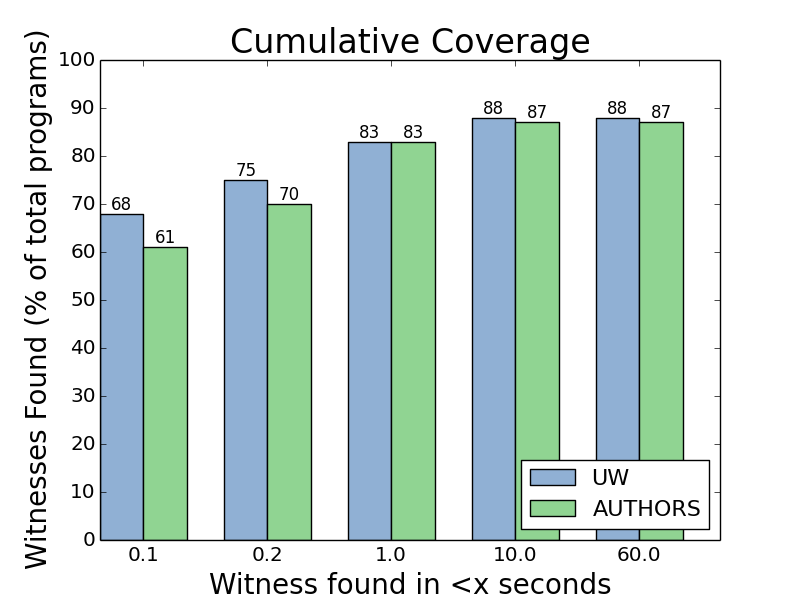
\includegraphics[width=\linewidth]{coverage.png}
\end{minipage}
\begin{minipage}{\linewidth}
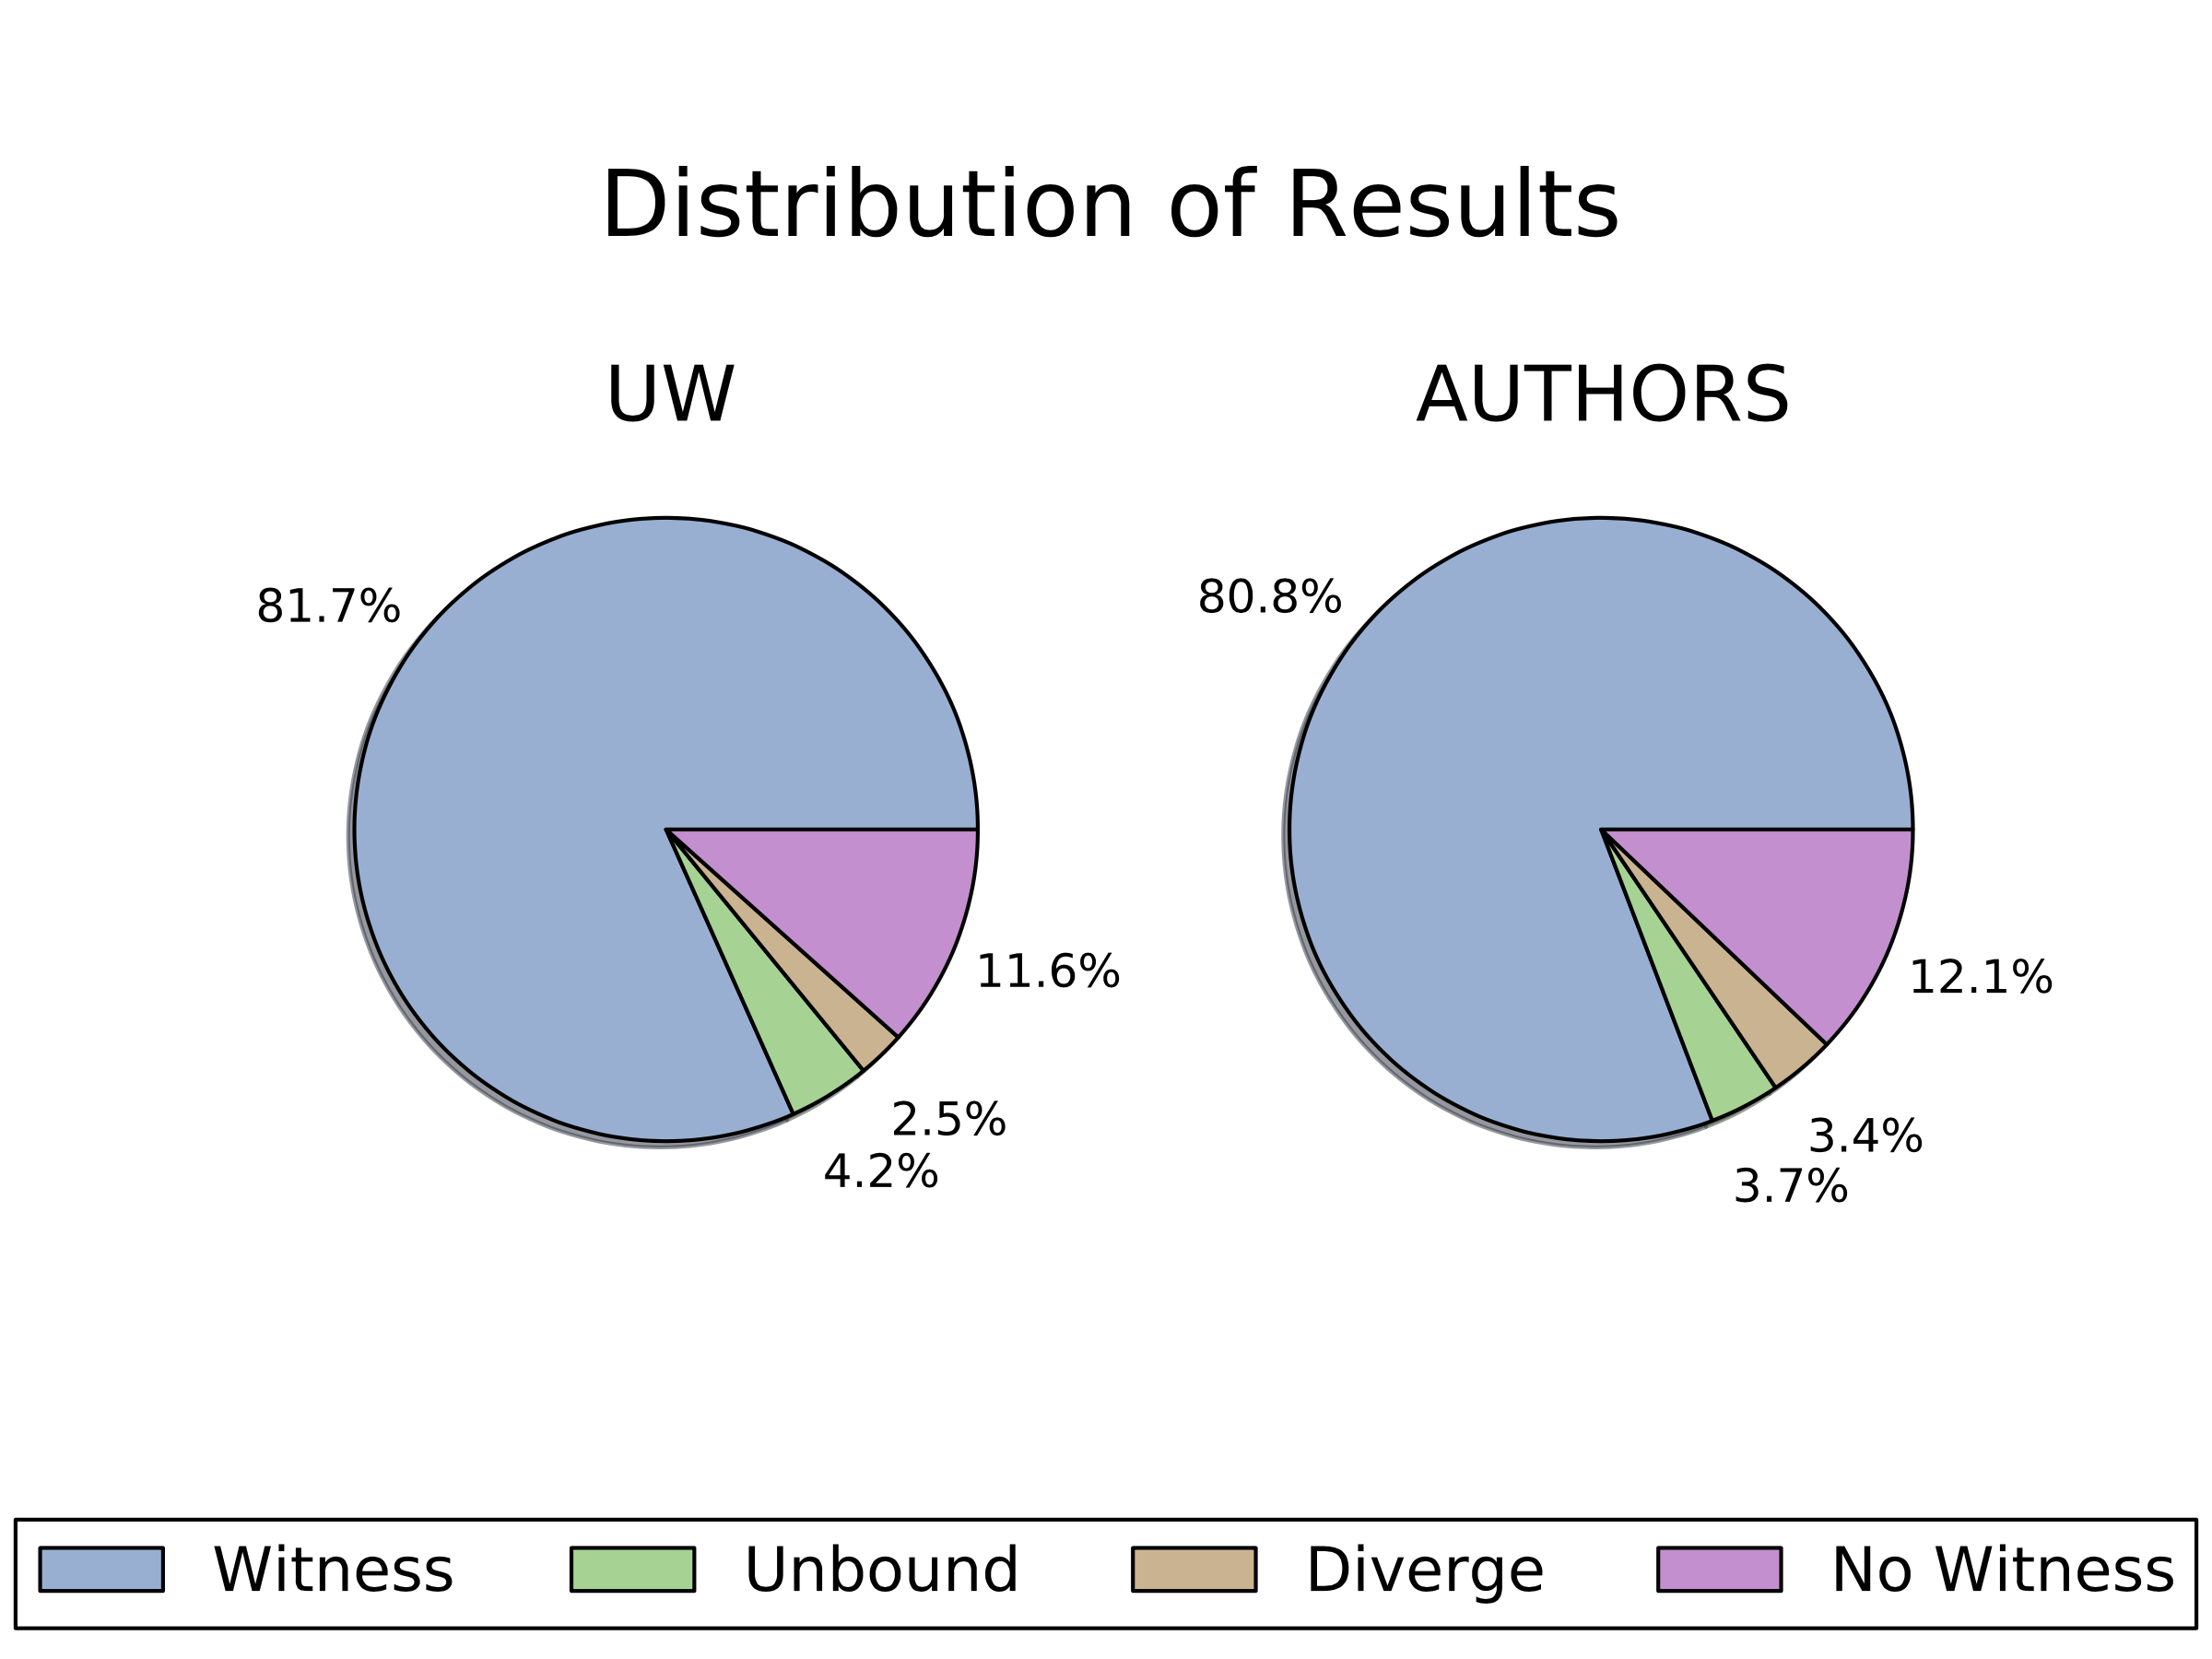
\includegraphics[width=\linewidth]{distrib.png}
\end{minipage}
% \vspace{-8ex}
\caption{Results of our coverage testing and the distribution of test
  outcomes. Our random search successfully finds witnesses for 83\% of
  the programs in under one second, improving slightly to 87\% in under
  10 seconds. In both datasets we detect actual type errors about 82\%
  of the time, unbound variables or constructors 3-4\% of the time, and
  diverging loops 2-3\% of the time. For the remaining 11-12\% of the
  programs we are unable to provide any useful feedback.  }
\label{fig:results-witness}
\end{figure}

\paragraph{Results}
\label{sec:results-witness}
The results of our experiments are summarized in
Figure~\ref{fig:results-witness}.
%
In both datasets our tool was able to find a witness for 83\% of the
programs in under one second, \ie fast enough to be integrated as a
compile-time check. If we extend our tolerance to a 10 second timeout,
we hit a maximum of 87\% coverage.
%
Interestingly, while the vast majority of witnesses corresponded to a
type-error, as expected, 3-4\% triggered an unbound variable error and
2-3\% triggered an infinite recursion error.
%
For the remaining 12\% of programs we were unable to provide any useful
feedback as they either completed 1,000 tests successfully, or timed out
after 10 minutes.
%
% XX programs were deemed safe and XX timed out even at 3,000 steps, \ie
% we could not provide any useful feedback for XX\% of the total programs.
%
While a more advanced search procedure, \eg dynamic-symbolic execution,
could likely trigger more of the type errors, our experiments show that
type errors are coarse enough (or that novice programs are \emph{simple}
enough) that these techniques are not necessary.


\subsection{Trace Complexity}
\label{sec:trace-complexity}

For each of the ill-typed programs for which we could
find a witness, we measure the complexity of the generated
trace according to two metrics.

\paragraph{Jump Compression}
%
A \emph{jump compressed} trace is one whose edges are limited to forward
or backward jumps. (The sizes of these traces is equal to the jump
metric below.)
%
In our experience, jump compression abstracts many details of the
computation that are often uninteresting or irrelevant to the
explanation.
% 
In particular, jump compressed traces hide low-level operations and
summarize function calls as call-return pairs, see
Figure~\ref{fig:fac-jump} for a variant of @fac@ that implements the
subtraction as a function call instead of a primitive.
%
\begin{figure}[t]
\centering
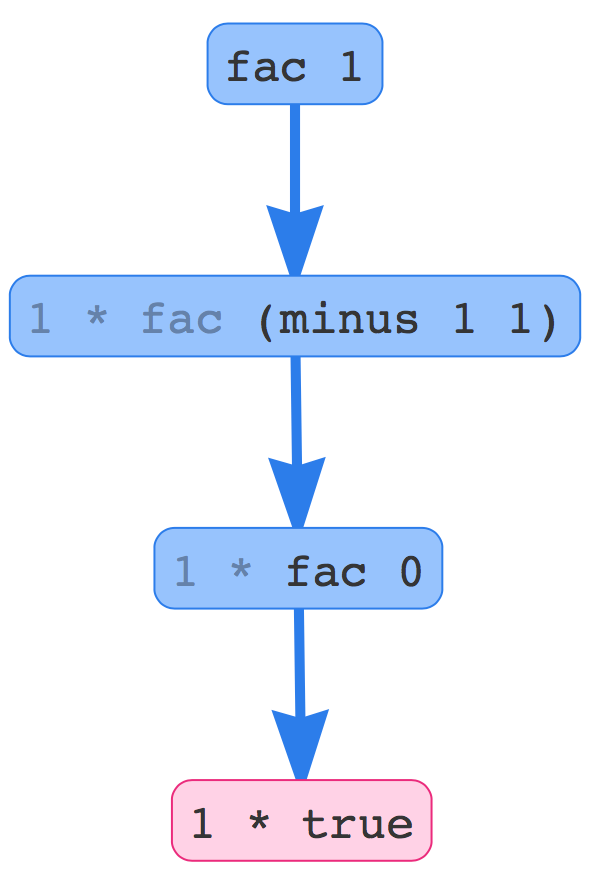
\includegraphics[height=2in]{fac-minus.png}
\caption{Jump-compressed trace of \texttt{fac 1} with subtraction
  implemented as a function call.}
\label{fig:fac-jump}
\end{figure}
%
Once the user has identified an interesting call-return pair, they can
step into the call and proceed with more fine-grained steps.
%
% Expanding the initial visualization to a jump-compressed trace is often
% an ideal first step;
% % expanding a jump-compressed traces ideal for the initial state of the
% they provide a concise overview of the execution and allow the user to
% step directly into an interesting function call, at which point the can
% proceed with more fine-grained steps.
%
Note that jump compressed traces are not quite the same as
stack-traces as they show \emph{all} function calls, including
those that returned successfully.
%
For example, the display on the right in Figure~\ref{fig:factorial} shows
a jump-compressed trace, of size 4. The full trace for
the same example has size 19.

\paragraph{Metrics} Thus, our two metrics are:
% size of the full trace,
% \ie the number of small-step reductions, and the size of the jump-compressed
% version of the trace.
%
\begin{enumerate}
\item \emphbf{Single-Step Metric}
      The number of single-step reductions along the path from the
      witness to the stuck term in the given witness execution, and
  % This can be thought of as a worst-case
  % complexity, \ie ``How big is the fully-expanded trace?''
\item \emphbf{Jump Metric}
      The size of the jump-compressed trace for the given witness execution,
      \ie\ the number of forward (or backward) jumps that can be taken along the
      path from the witness to the stuck term.
\end{enumerate}


% \item \ES{others?}
%
\begin{figure}[t]
\centering
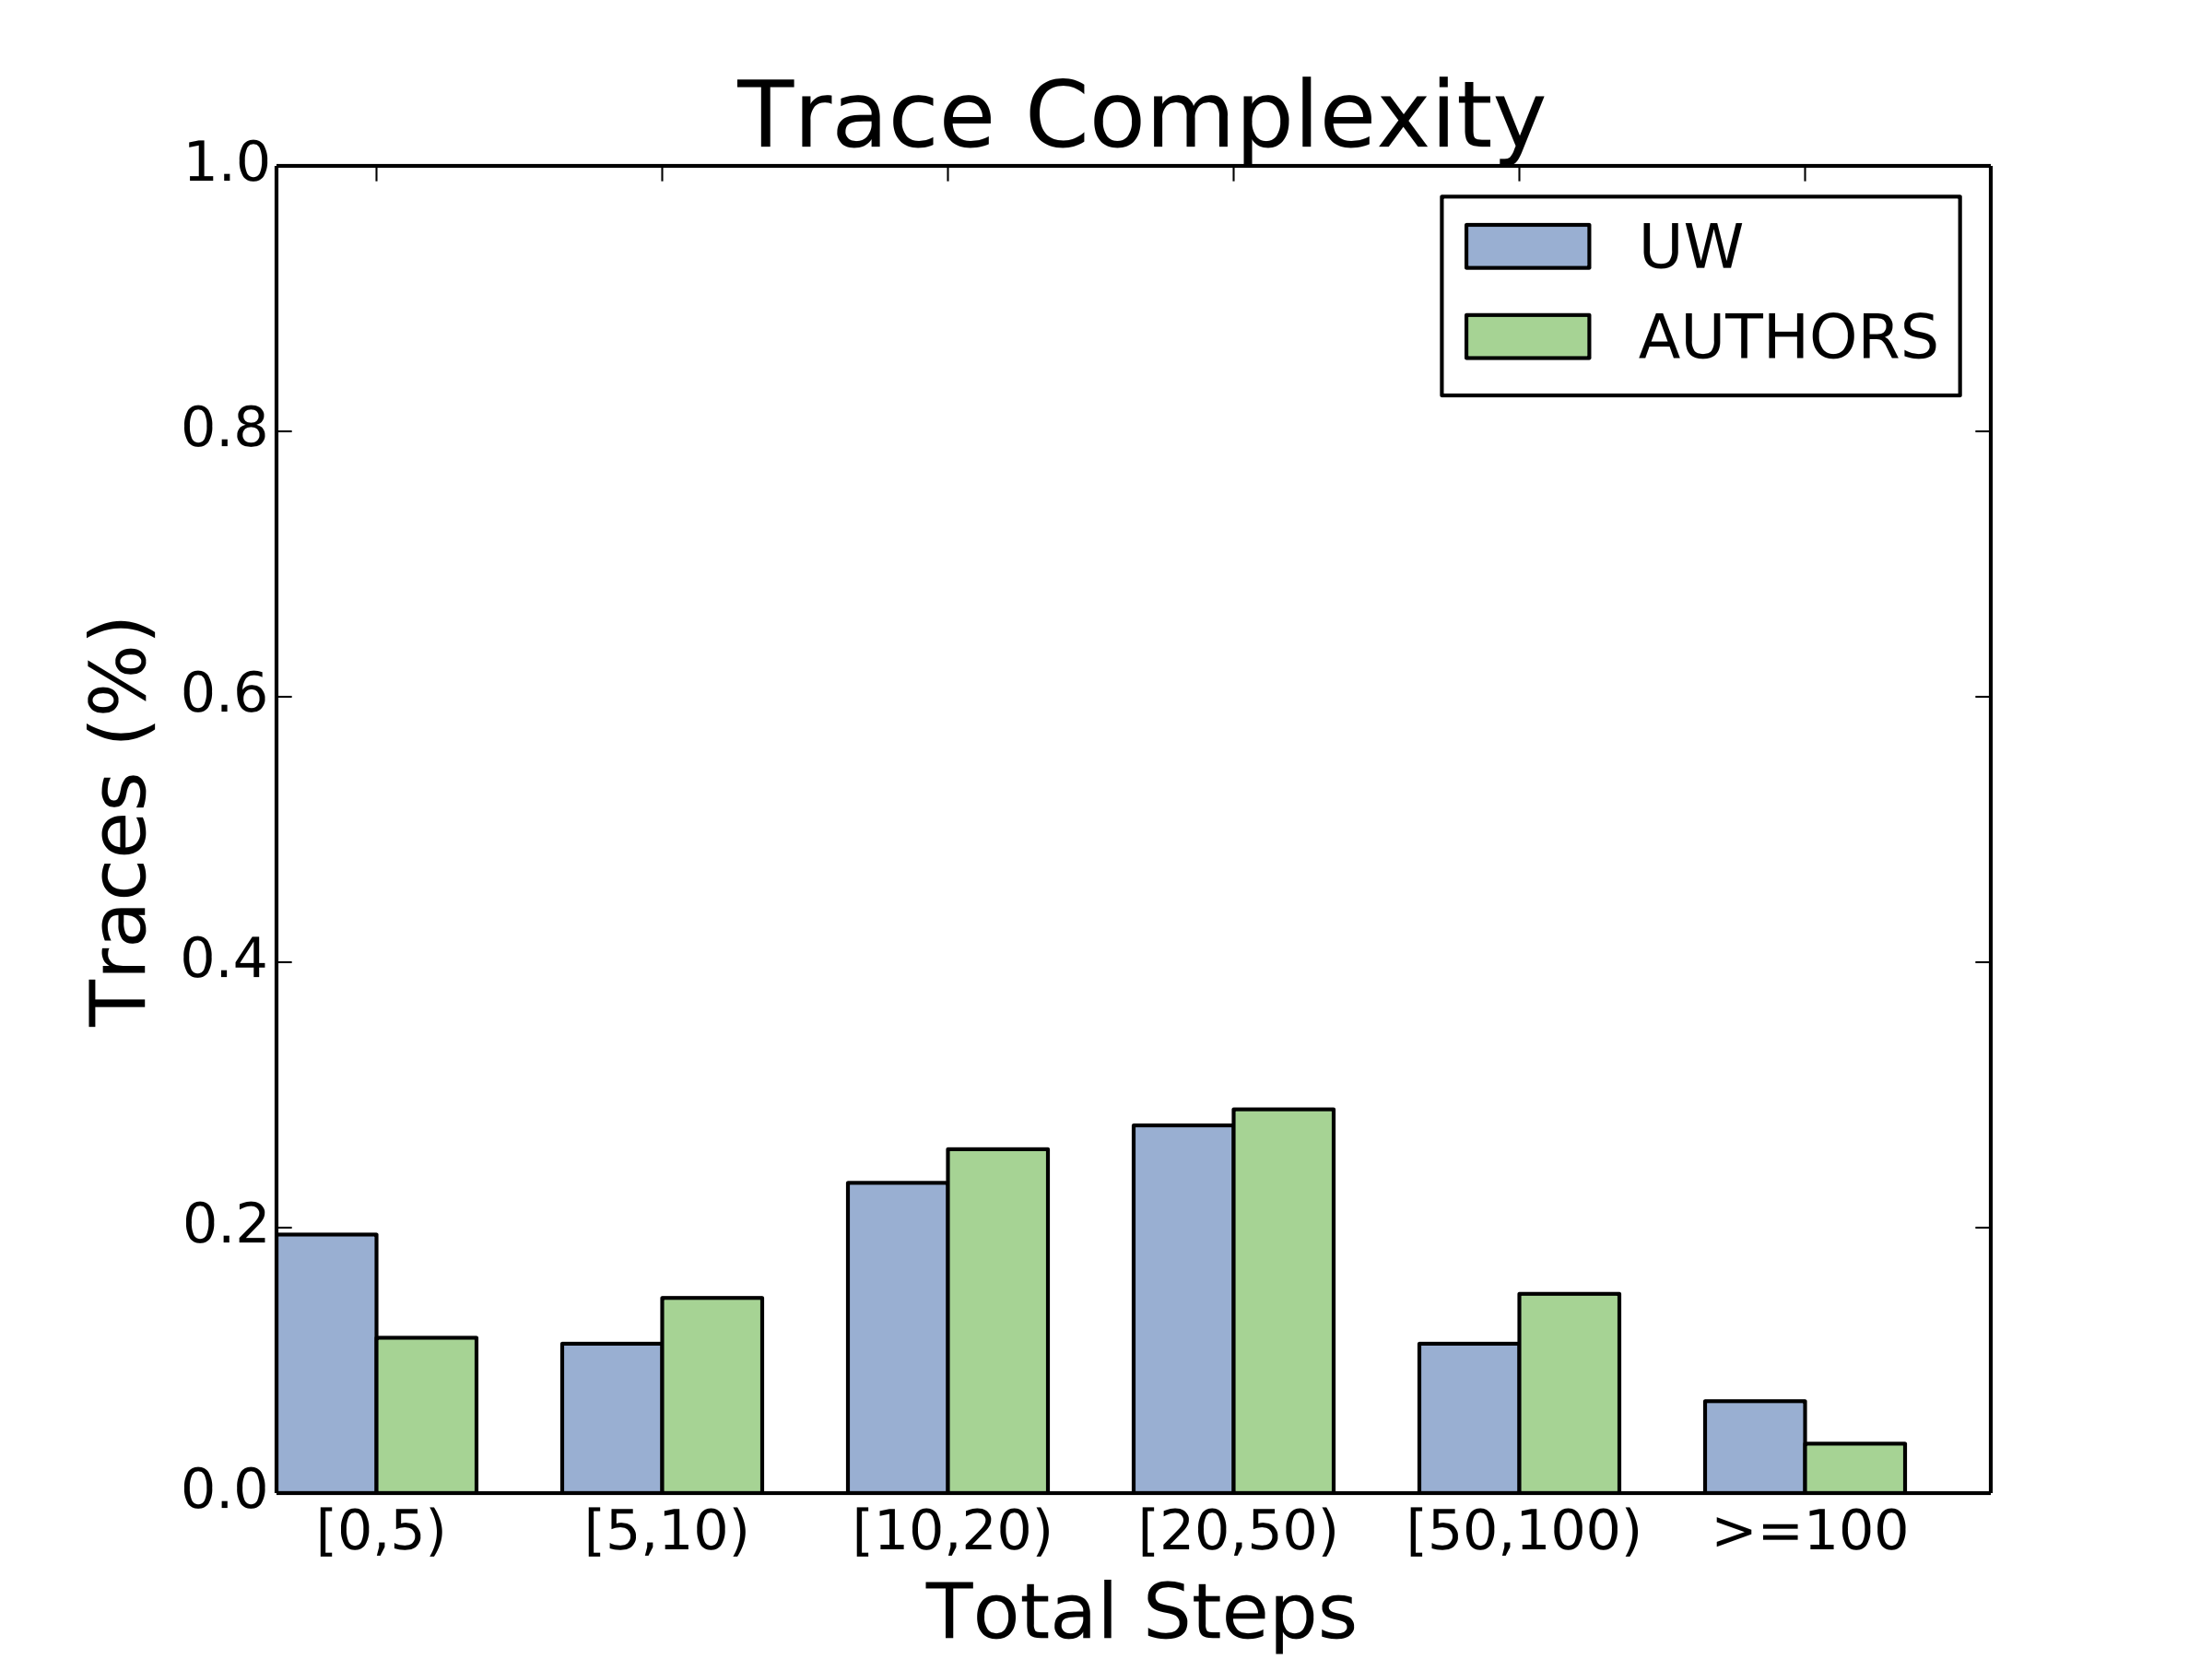
\includegraphics[width=\linewidth]{trace_size_step.png}
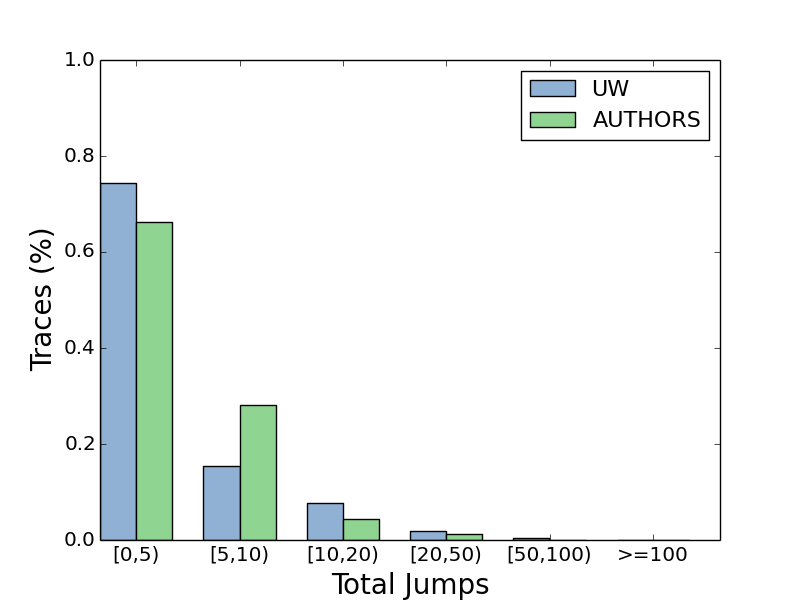
\includegraphics[width=\linewidth]{trace_size_jump.png}
\caption{Complexity of the generated traces. 81\% of the combined traces
  have a jump complexity of at most 10, with an average of 7 and a
  median of 5.}
\label{fig:results-complexity}
\end{figure}
%

\paragraph{Results}
\label{sec:results-complexity}
The results of the experiment are summarized in
Figure~\ref{fig:results-complexity}.
%
The average number of single-step reductions per trace is 31 for the
\ucsdbench\ dataset (35 for the \uwbench\ dataset) with a maximum of
2,745 (660 for \uwbench) and a median of 16 (also 16 for \uwbench).
%
The average number of jumps per trace is 7 (also 7 for \uwbench) with a
maximium of 353 (105 for \uwbench) and a median of 4 (also 4 for
\uwbench).
%
In both datasets at least 80\% of the traces contain at most 10 jumps.
%

\subsection{Discussion}
\label{sec:discussion}

To summarize, our experiments demonstrate that \nanomaly finds witnesses
to type errors: (1) with high coverage in a timespan amenable to
compile-time analysis, and (2) with traces that have a low average
complexity of 3 function calls.

There are, of course, drawbacks to our approach. Three that stand out
are: (1) coverage limits due to random generation, (2) the inability to
handle certain instances of infinite types, and (3) dealing with an
explosion in the size of generated traces.

\paragraph{Random Generation}
Random test generation has difficulty generating highly constrained
values, \eg red-black trees or a pair of equal integers. If the type
error is hidden behind a complex branch condition \nanomaly may not be
able to trigger it. Exhaustive testing and dynamic-symbolic execution
can address this short-coming by performing an exhaustive search for
inputs (\emph{resp}. paths through the program). As our experiments
show, however, novice programs do not appear to require more advanced
search techniques, likely because the novice programs tend to be simple.

\paragraph{Infinite Types}
Our implementation does check for infinite types inside \forcesym, but
there are some degenerate cases where it is unable to detect
them. Consider, for example, the following buggy version of @replicate@.
% ,
% which is supposed to produce a list containing @n@ copies of @x@.
%
\begin{code}
  let rec replicate n x =
    if n <= 0 then
      []
    else
      replicate (n-1) [x]
\end{code}
%
This code produces a nested list (with @n@ levels of nesting) containing
a single copy of @x@, instead of a list with @n@ copies of @x@. \ocaml
detects a cyclic \hbox{@'a = 'a list@} constraint in the recursive call
and throws a type error, whereas \nanomaly happily % recurses @n@ times to
produces the nested list.  Strictly speaking, this function itself cannot
``go wrong'', the program would not get stuck until a \emph{client}
attempted to use the result expecting a flat list. But this is not very
satisfying as @replicate@ is clearly to blame. Furthermore, in our
experience, infinite-type errors are often difficult to %some of the more difficult ones to
debug (and to explain to novices), so better support for this scenario
would be useful.

\paragraph{Trace Explosion}
Though the average complexity of our generated traces is low in terms of
jumps, there are some extreme outliers. We cannot reasonably expect a
novice user to explore a trace containing 50+ terms and draw a
conclusion about which pieces contributed to the bug in their
program. Enhancing our visualization to slice out program paths relevant
to specific values, \eg\ in the style of~\cite{perera_functional_2012},
would likely help alleviate this issue, allowing users to
highlight a confusing value and ask: ``Where did this come from?''


% \begin{itemize}
% \item benchmarks: our data + seminal data
% \item both cases: \textbf{random} search sufficient to trigger runtime crash in 80\% of programs
% \item how many of the ``safe'' programs are actually safe??
% \end{itemize}

%%% Local Variables: 
%%% mode: latex
%%% TeX-master: "main"
%%% End: 
